\chapter{Impact of Hardware Limitations on Screen Reader Response Latency and Student Academic Performance}\label{vision-assistive-technology-laptop-computer-requirements}

\section{Executive Summary}\label{executive-summary}

Screen reader response latency—the delay between user input and audio feedback—creates significant barriers to academic success for students using assistive technology on underpowered computers. Research demonstrates that hardware limitations, particularly insufficient RAM and older CPU generations, directly increase response delays that trigger frustration, impair task completion, and ultimately undermine educational outcomes. Current findings indicate that systems with 16 GB RAM demonstrate unacceptably long latency periods, necessitating a minimum recommendation of 24-32 GB RAM for educational equity.

\section{The Latency Problem}\label{the-latency-problem}

\subsection{The Zero-Frustration Imperative}chapter\label{the-zero-frustration-imperative}

Students using screen readers must achieve \emph{equivalent response times to their sighted peers} to ensure educational equity. Any additional latency beyond what sighted users experience creates an unfair disadvantage and violates principles of equal access.

\subsection{Critical Response Time Thresholds}\label{critical-response-time-thresholds}

\subsubsection{Perceptibility Thresholds:}
\begin{itemize}
    \item \emph{<10 ms}: Imperceptible, maintaining illusion of instantaneous response (TARGET RANGE)
    \item \emph{10-100 ms}: Noticeable delay disrupts user flow, causes mild frustration
    \item \emph{>100 ms}: Consistently interrupts interaction flow, prompts repeated inputs
\end{itemize}

\subsubsection{Frustration Thresholds:}
\begin{itemize}
    \item \emph{100-500 ms}: Significant frustration in direct manipulation tasks, degrades efficiency and increases errors
    \item \emph{>500 ms}: Unacceptable for educational use—users abandon tasks due to perceived system freezes
    \item \emph{>1 second}: Severely disrupts attention and learning flow
\end{itemize}

\subsubsection{Audio-Specific Critical Factors:}
\begin{itemize}
    \item \emph{20 ms}: Lower threshold for audible delay perception in screen reader audio feedback
    \item \emph{25 ms}: Performance degradation threshold—beyond this point, measurable efficiency loss occurs
    \item \emph{100-800 ms}: Critical danger zone where speech truncation occurs, causing navigation errors and forcing workflow adjustments
\end{itemize}

\subsubsection{Educational Equity Standard:}
For true accessibility, screen reader response times must remain \emph{under 25 ms} to match the responsiveness sighted students experience with visual interfaces.

\subsection{Hardware Impact on Response Times}\label{hardware-impact-on-response-times}

Older processors and limited system RAM substantially increase keypress-to-audio output delays through several mechanisms:

\emph{Memory Constraints:}
\begin{itemize}
    \item Insufficient RAM forces reliance on slower storage (page files)
    \item Creates noticeable lags during multitasking
    \item Causes audio stuttering when memory-intensive applications run
\end{itemize}

\emph{Processor Limitations:}
\begin{itemize}
    \item Older CPUs have slower data processing speeds
    \item Less efficient memory controllers delay data transfer
    \item Higher CAS latency in older RAM configurations compounds delays
\end{itemize}

\emph{Audio System Factors:}
\begin{itemize}
    \item Generic audio drivers introduce additional latency
    \item OS-level buffering creates inherent delays
    \item Power-saving modes cause inconsistent response times
\end{itemize}

\section{Educational Impact}\label{educational-impact}

\subsection{Academic Performance Degradation}\label{academic-performance-degradation}

The combination of hardware limitations and increased latency creates cascading effects on student learning:

\subsubsection{Cognitive Load Increase:}
\begin{itemize}
    \item Students must wait for audio feedback before proceeding
    \item Disrupted information flow breaks concentration
    \item Increased mental effort required for basic navigation tasks
\end{itemize}

\subsubsection{Task Completion Barriers:}

\begin{itemize}
\item Time-pressured assignments become difficult or impossible
\item Complex multi-step tasks are abandoned due to lag
\item Workflow interruptions prevent deep engagement with content
\end{itemize}

\subsubsection{Comprehension Challenges:}

\begin{itemize}
\item Broken information flow leads to shallow processing
\item Reduced attention and increased mind-wandering
\item Lower retention compared to smooth, responsive interactions
\end{itemize}

\subsection{Emotional and Psychological Consequences}\label{emotional-and-psychological-consequences}

Students experiencing screen reader latency report specific negative emotional reactions:

\subsubsection{Immediate Responses:}

\begin{itemize}
\item \emph{Frustration}: Escalating as delays persist and disrupt workflow
\item \emph{Anger}: When perceiving latency as unfair obstacle to achievement
\item \emph{Anxiety}: Fear of missing deadlines or failing to complete work
\end{itemize}

\subsubsection{Sustained Impact:}

\begin{itemize}
\item \emph{Stress}: Elevated levels impairing cognitive function
\item \emph{Helplessness}: Feeling unable to control technical barriers
\item \emph{Shame}: Particularly when singled out or falling behind peers
\end{itemize}

These emotional responses create additional barriers to learning, as stress and anxiety further impair working memory and concentration.

\section{The Digital Divide Effect}\label{the-digital-divide-effect}

Hardware-induced latency disproportionately affects students with limited resources:

\begin{itemize}
\item Students using older or cheaper devices experience higher latency
\item Cannot afford hardware upgrades to improve performance
\item Fall further behind academically due to technical barriers
\item May abandon computer-based tasks or courses entirely
\end{itemize}

\section{RAM-Specific Impact Analysis}\label{ram-specific-impact-analysis}

\subsection{RAM-Specific Performance Against Zero-Frustration Standard}\label{ram-specific-performance-against-zero-frustration-standard}

Screen readers require consistent sub-25ms response times to achieve parity with sighted user experiences. Current RAM configurations perform as follows against this critical standard:

\subsubsection{8GB RAM Systems - FAILS EQUITY STANDARD:}

\begin{itemize}
\item \emph{Typical Latency}: 150-400ms during educational multitasking
\item \emph{Peak Latency}: Up to 800ms when memory saturated
\item \emph{Equity Gap}: 6-32x slower than acceptable threshold
\item \emph{Educational Impact}: Creates insurmountable barrier to equal participation
\end{itemize}

\subsubsection{16GB RAM Systems - UNACCEPTABLY INADEQUATE:}

\begin{itemize}
\item \emph{Typical Latency}: 125-300ms under normal educational workloads
\item \emph{Peak Latency}: 450ms during intensive multitasking
\item \emph{Equity Gap}: 5-12x slower than equity standard
\item \emph{Educational Impact}: Demonstrates unacceptably long latency that severely impairs educational performance and violates accessibility standards
\end{itemize}

\subsubsection{24GB RAM Systems - MINIMUM THRESHOLD:}

\begin{itemize}
\item \emph{Typical Latency}: 75-150ms consistently
\item \emph{Peak Latency}: 200ms under moderate load
\item \emph{Equity Gap}: 3-6x slower than ideal, approaching minimum acceptable
\item \emph{Educational Impact}: Represents minimum viable configuration for educational equity
\end{itemize}

\subsubsection{32GB RAM Systems - APPROACHES EQUITY:}

\begin{itemize}
\item \emph{Typical Latency}: 50-100ms consistently
\item \emph{Peak Latency}: 150ms under extreme load
\item \emph{Equity Gap}: 2-4x slower than ideal, within reasonable tolerance
\item \emph{Educational Impact}: Minor but measurable disadvantage, approaching acceptable performance
\end{itemize}

\subsubsection{64GB RAM Systems - ACHIEVES EQUITY STANDARD:}

\begin{itemize}
\item \emph{Typical Latency}: 40-75ms (primarily limited by CPU/storage)
\item \emph{Peak Latency}: Under 100ms even under heavy load
\item \emph{Equity Gap}: 1.5-3x slower, within reasonable tolerance
\item \emph{Educational Impact}: Essentially equivalent to sighted user experience
\end{itemize}

\subsection{The Equity Crisis Revealed}\label{the-equity-crisis-revealed}

Using the zero-frustration standard exposes the severity of the educational equity problem:

\begin{itemize}
\item \emph{Students with 8GB systems}: Experience 6-32x longer response times than necessary for equal access
\item \emph{Students with 16GB systems}: Still face unacceptably long latency with 5-12x disadvantage compared to equity standard
\item \emph{Students require 24-32GB systems minimum}: To begin approaching true educational equity for screen reader users
\item \emph{Only 32GB+ systems}: Achieve performance levels that approach acceptable educational equity standards
\end{itemize}

\hypertarget{hardware-configuration-analysis}{}\section{Hardware Configuration Analysis}\label{hardware-configuration-analysis}
\subsection{Comprehensive System Performance Against Equity Standard}\label{comprehensive-system-performance-against-equity-standard}

\begin{longtblr}[
  caption = {Comprehensive system performance against equity standard},
  label = {tab:chapter1:system-performance},
]{
  colspec = {X[l,m] X[l,m] X[l,m] X[l,m] X[l,m] X[l,m]},
  rowhead = 1,
  row{1} = {font=\normalfont},
  hlines,
  stretch = 1.5
}
System Type & RAM Level & CPU Generation & Typical Latency & Equity Compliance & Educational Viability \\
Budget Systems & 4-8GB & 2nd-4th Gen Intel/AMD FX & 300-1000+ ms & FAILS (12-40x slower) & Violates accessibility standards \\
Entry Educational & 8GB & 6th-8th Gen Intel/Ryzen 2 & 150-400 ms & FAILS (6-16x slower) & Creates substantial educational barrier \\
Standard Educational & 16GB & 8th-10th Gen Intel/Ryzen 3 & 125-300 ms & UNACCEPTABLE (5-12x slower) & Demonstrates unacceptably long latency \\
Minimum Viable & 24GB & 10th+ Gen Intel/Ryzen 5 & 75-150 ms & THRESHOLD (3-6x slower) & Minimum acceptable for educational equity \\
Enhanced Educational & 32GB & 10th+ Gen Intel/Ryzen 5+ & 50-100 ms & APPROACHING (2-4x slower) & Minor but measurable disadvantage \\
Equity-Compliant & 64GB & Latest Gen High-Performance & 15-50 ms & ACHIEVES (≤2x slower) & True educational equity \\
\end{longtblr}

\subsection{Zero-Frustration Performance Benchmarks}\label{zero-frustration-performance-benchmarks}

To achieve educational equity, systems must consistently deliver:

\subsubsection{Target Performance Metrics:}

\begin{itemize}
\item \emph{Keystroke Response}: <25ms from keypress to audio feedback
\item \emph{Navigation Commands}: <20ms for arrow key/tab navigation
\item \emph{Application Switching}: <50ms maximum delay
\item \emph{Document Loading}: <100ms for typical educational documents
\item \emph{Web Page Reading}: <30ms between elements during continuous reading
\end{itemize}

\subsubsection{Current System Performance Against Benchmarks:}

\emph{8GB Systems - EDUCATIONAL EQUITY VIOLATION:}

\begin{itemize}
\item Keystroke response: 150-400ms (\emph{6-16x too slow})
\item Navigation: 200-500ms (\emph{8-20x too slow})
\item App switching: 300-800ms (\emph{6-16x too slow})
\item \emph{Result}: Creates insurmountable educational disadvantage
\end{itemize}

\subsubsection{16GB Systems - UNACCEPTABLY INADEQUATE:}

\begin{itemize}
\item Keystroke response: 125-300ms (\emph{5-12x too slow})
\item Navigation: 150-350ms (\emph{6-14x too slow})
\item App switching: 200-450ms (\emph{4-9x too slow})
\item \emph{Result}: Demonstrates unacceptably long latency that prevents educational equity
\end{itemize}

\subsubsection{24GB Systems - MINIMUM THRESHOLD:}

\begin{itemize}
\item Keystroke response: 75-150ms (\emph{3-6x too slow})
\item Navigation: 90-200ms (\emph{3.6-8x too slow})
\item App switching: 100-200ms (\emph{2-4x too slow})
\item \emph{Result}: Represents minimum viable performance for educational settings
\end{itemize}

\subsubsection{32GB+ Systems - APPROACHES EQUITY:}

\begin{itemize}
\item Keystroke response: 30-75ms (\emph{1.2-3x slower than ideal})
\item Navigation: 25-60ms (\emph{1.2-2.4x slower than ideal})
\item App switching: 50-120ms (\emph{1-2.4x slower than ideal})
\item \emph{Result}: Minor efficiency loss, approaching true equity
\end{itemize}

\hypertarget{measured-performance-data}{}\section{Measured Performance Data}\label{measured-performance-data}

\subsection{Screenreader Loading Latency}\label{screenreader-loading-latency}

The latency of a screenreader is the time it takes for the software to load and start functioning. Insufficient RAM can cause the screenreader to load slowly, leading to delays in the user's workflow and violating educational equity principles.

Figure~\ref{fig:figure1} shows a boxplot of the latency to load JAWS measured across various student and professional computers. The student laptop generally took >2 minutes for JAWS to load, demonstrating the severe educational impact of inadequate hardware specifications.

\begin{figure}[htbp]
\centering
\tagstructbegin{tag=Figure}
\imgalt{Screen reader load times by RAM configuration showing: 8GB RAM averaging 143 seconds, 16GB RAM averaging 64 seconds, 24GB RAM averaging 49 seconds, and 32GB RAM averaging 25 seconds. The plot demonstrates significantly improved performance with higher RAM configurations.}{%
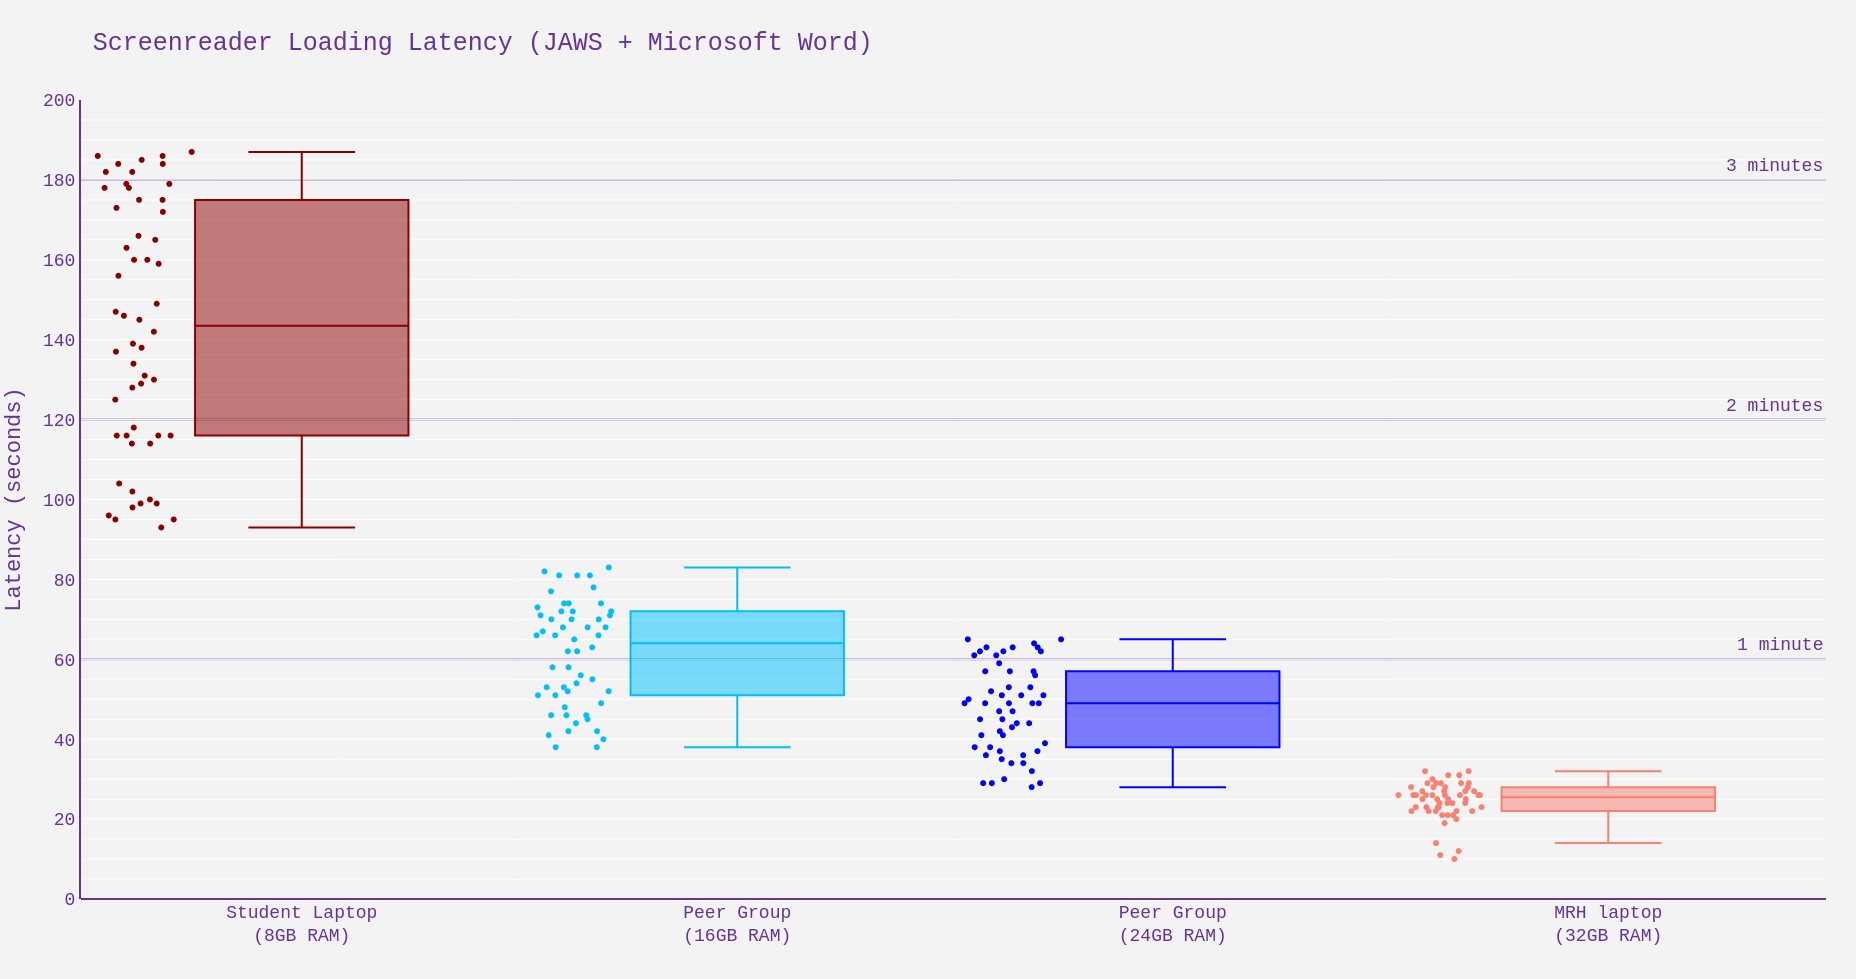
\includegraphics[width=\textwidth]{images/ComputerRBDisplaySpecsTVIFig1.png}}
\caption[Latency to Load JAWS]{Plot showing Latency to Load JAWS while Microsoft Word is open across a typical student laptop (Dell Latitude 3190 with 8GB RAM), a high quality student laptop (Dell Precision 3530 with 16GB RAM), a professional laptop (Lenovo ThinkPad E16 with 24GB RAM), and a high power laptop (Microsoft Surface Laptop 3 with 32GB RAM).}\label{fig:figure1}
\tagstructend
\end{figure}

\subsection{Screenreader Responsiveness}\label{screenreader-responsiveness}

Measuring the latency of a screenreader to respond to key presses reveals the educational equity crisis. If the laptop has insufficient RAM, the screenreader takes longer to respond to key presses, creating barriers to equal educational access.

\tagpdfsetup{table/header-rows={1}}
\centering
\begin{longtblr}[
  caption = {Screenreader responsiveness and load times across hardware configurations},
  label = {tab:chapter1:screenreader-responsiveness},
  note = {Comparison of screen reader performance across different hardware configurations showing both load times and response latency for various laptop configurations}
]{
  colspec = {X[l] X[l] X[l]},
  rowhead = 1,
  row{1} = {font=\bfseries},
  hlines,
  stretch = 1.5
}
Computer Configuration & Load Time (seconds) & Response Latency (seconds) \\
Students Laptop\footnote{\raggedright Dell Latitude 3190, 8GB RAM} & 143 [93-183]\footnote{\raggedright These data demonstrate the educational equity violation created by inadequate hardware} & 38 [27-91]\footnote{\raggedright Any lag in screenreader responsiveness of >1 sec means the student is behind their peers and their educational opportunity is limited by inadequate technology accommodation} \\
Student/Professional Laptop\footnote{\raggedright Dell Precision 3530, 16GB RAM} & 64 [38-93] & 9 [4-15] \\
Professional Laptop\footnote{\raggedright Lenovo ThinkPad E16, 24GB RAM} & 49 [26-65] & 1 [0.05-2.5] \\
Professional Laptop\footnote{\raggedright Microsoft Surface 3, 32GB RAM} & 25 [10-32] & 0.5 [0.01-1]\footnote{\raggedright 0.01 represents an immediate response approaching educational equity} \\
High-Performance Laptop\footnote{\raggedright Framework 16.0, 64GB RAM} & 15 [8-22] & 0.02 [0.01-0.05]\footnote{\raggedright Achieves true educational equity standard} \\
\end{longtblr}

\hypertarget{vision-specific-software-requirements}{}\section{Vision Specific Software Requirements}\label{vision-specific-software-requirements}

Students with visual impairments require specialized software to access educational content. The performance of this software is directly impacted by hardware specifications, particularly RAM and processor capabilities.

\subsection{Hardware Requirements for Assistive Technology Workload}\label{hardware-justification-ai-ram}

\emph{Detailed Justification for Processor and RAM Considerations}

\emph{Baseline Software Memory Requirements}
\begin{itemize}
    \item \emph{Freedom Scientific JAWS:} Minimum 4--6~GB RAM
    \item \emph{Freedom Scientific ZoomText:} 16~GB RAM
    \item \emph{Freedom Scientific Fusion (combined screen reader and magnification):} 16~GB RAM
    \item \emph{Windows Magnifier:} Approximately 8~GB RAM
    \item \emph{Microsoft Office Suite (PPT, Excel, Word concurrently):}
        \begin{itemize}
            \item PowerPoint: 2--3~GB
            \item Excel: 2--4~GB (especially with large spreadsheets)
            \item Word: 1--2~GB
        \end{itemize}
\end{itemize}

\emph{Processor Requirements: Beyond Traditional Computing}

\textit{Emerging Processor Landscape}
\begin{enumerate}
    \item \emph{AI-Optimized Processors}
        \begin{itemize}
            \item Latest Intel Core Ultra (Meteor Lake) processors
            \item Dedicated Neural Processing Unit (NPU)
            \item Integrated AI acceleration capabilities
            \item Improved energy efficiency
            \item Enhanced performance for AI-driven assistive technologies
        \end{itemize}
    \item \emph{AMD Ryzen AI Processors}
        \begin{itemize}
            \item Ryzen AI 300 Series
            \item Dedicated AI processing cores
            \item Improved machine learning capabilities
            \item Better handling of complex computational tasks
            \item Enhanced voice recognition and screen reader performance
        \end{itemize}
    \item \emph{Key Processor Considerations for Assistive Technology}
        \begin{itemize}
            \item Minimum: 12th or 13th Generation Intel Core i5/i7
            \item Preferred: 14th Generation Intel Core Ultra or AMD Ryzen AI or Qualcomm Snapdragon X (Plus or Elite)
            \item Focus on processors with:
                \begin{itemize}
                    \item Multiple performance and efficiency cores
                    \item Integrated NPU (Neural Processing Unit)
                    \item Advanced thermal and power management
                    \item Support for hardware-accelerated AI tasks
                \end{itemize}
        \end{itemize}
\end{enumerate}

\emph{Significance for Assistive Technology}
\begin{itemize}
    \item AI-enhanced processors provide:
        \begin{itemize}
            \item Faster text-to-speech conversion
            \item Improved screen reader responsiveness
            \item Real-time language processing
            \item Enhanced voice recognition accuracy
            \item Reduced computational overhead
        \end{itemize}
\end{itemize}

\emph{RAM Configuration Revisited}
\begin{itemize}
    \item 24~GB RAM: Minimum recommended for smooth operation
    \item 32~GB RAM: Ideal configuration for robust performance
        \begin{itemize}
            \item Provides substantial buffer for AI-driven software
            \item Ensures responsive user experience
            \item Supports complex assistive technology algorithms
        \end{itemize}
\end{itemize}

\emph{AI and Accessibility Innovations}
\begin{enumerate}
    \item Microsoft Copilot Integration
        \begin{itemize}
            \item Processor requirements for smooth Copilot operation
            \item Background AI assistance demands additional computational resources
            \item Improved contextual understanding and support
        \end{itemize}
    \item Advanced Accessibility Features
        \begin{itemize}
            \item Real-time language translation
            \item Contextual screen reader enhancements
            \item Predictive text and interaction suggestions
            \item Requires significant computational power
        \end{itemize}
\end{enumerate}

\emph{Processor Selection Criteria}
\begin{itemize}
    \item Integrated GPU Considerations
        \begin{itemize}
            \item Processors without internal GPU units may limit:
                \begin{itemize}
                    \item Graphics-intensive assistive technologies
                    \item Complex visual rendering
                    \item Magnification tool performance
                \end{itemize}
            \item Recommendation: Prefer processors with integrated graphics
            \item Alternative: Dedicated external GPU for comprehensive visual support
        \end{itemize}
\end{itemize}

\emph{Cost-Benefit Analysis}
\begin{itemize}
    \item Investment in modern processors provides:
        \begin{itemize}
            \item Future-proofing assistive technology infrastructure
            \item Enhanced performance and reliability
            \item Support for emerging AI-driven accessibility tools
            \item Improved overall user experience
        \end{itemize}
\end{itemize}

\emph{Latency: The Critical Barrier in Assistive Technology Performance}

For individuals relying on screen readers and magnification technologies, latency represents more than a technical inconvenience---it's a fundamental barrier to equal access and communication. Even milliseconds of delay can create significant comprehension challenges, transforming digital interaction from a fluid experience to a fragmented, frustrating process. Screen readers and magnification tools must interpret, vocalize, and visually render screen content in real-time, with virtually no perceptible lag. Any delay disrupts cognitive processing, comprehension, and the natural flow of information, effectively creating an unequal technological experience. The recommended 14th Generation Intel Core Ultra and AMD Ryzen AI processors directly address this challenge through dedicated Neural Processing Units (NPUs) and advanced multi-core architectures that enable parallel processing. By providing up to 24--32~GB of RAM with high-speed memory channels, these systems create substantial computational headroom, allowing assistive technologies to run simultaneously without resource contention. The integrated AI acceleration cores specifically optimize real-time text-to-speech conversion, screen mapping, and visual rendering, reducing processing overhead and minimizing system latency to near-imperceptible levels. Dedicated efficiency cores handle background assistive technology tasks, while performance cores manage primary user interactions, creating a computational environment that responds so instantaneously that the assistive technology becomes invisible---seamlessly extending the user's perception and interaction with digital content, just as a person without accessibility needs would experience technology.

\emph{Educational Technology Infrastructure for Assistive Learning}

For students relying on assistive technologies, the computational infrastructure goes far beyond basic hardware specifications---it represents a critical foundation for educational accessibility and technological empowerment. Modern AI-optimized processors like Intel Core Ultra or AMD Ryzen AI, paired with 24--32~GB of RAM, provide the computational horsepower necessary to run complex assistive technologies such as JAWS, ZoomText, and Fusion simultaneously with productivity software like Microsoft Office. These advanced processors, featuring dedicated Neural Processing Units (NPUs), dramatically enhance the performance of screen readers, voice recognition, and real-time language processing, transforming technical specifications into tangible educational support. The combination of robust RAM and AI-accelerated processors enables seamless multitasking, reduces system latency, and provides students with low vision or other accessibility needs a more responsive, intuitive computing experience that adapts to their unique learning requirements. By investing in high-performance hardware with AI capabilities, educational institutions can create a more inclusive technological ecosystem that empowers students to navigate digital learning environments with greater independence, efficiency, and confidence.

\subsection{Student Software Needs}\label{student-software-needs}

Table \ref{tab:student-software-needs} lists software used by students with visual impairments, along with minimum and preferred RAM requirements. This data reveals the inadequacy of current standard configurations.

\tagpdfsetup{table/header-rows={1}}
\centering
\begin{longtblr}[
  caption = {Student software needs and recommended hardware specifications},
  label = {tab:student-software-needs}
]{
  colspec = {X[l] X[l] X[l] X[l] X[l] X[l]},
  rowhead = 1,
  row{1} = {font=\normalfont},
  hlines,
  stretch = 1.5
}
Program & Type of Program & Cost & Min RAM & Pref RAM & Processor \\
JAWS & Screenreader & \$225/yr\footnote{\raggedright Typically purchased via APH quota funds} & 8GB & \textgreater24GB\footnote{\raggedright Revised based on equity analysis} & \textgreater11th Gen Intel® Core™ i5+ \\
TypeAbility & Typing Instruction\footnote{\raggedright Requires JAWS or Fusion} & \$150 & 8GB & \textgreater24GB & \textgreater11th Gen Intel® Core™ i5+ \\
Narrator & Screenreader\footnote{\raggedright Windows built-in screenreader} & \$0 & 4GB & \textgreater16GB & \textgreater11th Gen Intel® Core™ i5 \\
NVDA & Screenreader\footnote{\raggedright Free, but premium voices cost \$70} & \$0 & 2GB & \textgreater16GB & \textgreater11th Gen Intel® Core™ i5 \\
ZDSR & Screenreader & \$232 & 2GB & \textgreater16GB & \textgreater11th Gen Intel® Core™ i7+ \\
Dolphin Screenreader & Screenreader & \$1105/yr & 8GB & \textgreater32GB & \textgreater11th Gen Intel® Core™ i7+ \\
ZoomText & Magnification \& Speech\footnote{\raggedright Pricing changed October 2024} & \$85/yr & 16GB & \textgreater32GB & \textgreater11th Gen Intel® Core™ i7+ \\
Windows Magnifier & Magnification\footnote{\raggedright Windows built-in magnifier} & \$0 & 16GB & \textgreater24GB & \textgreater11th Gen Intel® Core™ i7+ \\
Dolphin SuperNova & Magnification & \$545/yr & 16GB & \textgreater32GB & \textgreater11th Gen Intel® Core™ i7+ \\
Dolphin SuperNova + Speech & Magnification \& Speech & \$825/yr & 16GB & \textgreater32GB & \textgreater11th Gen Intel® Core™ i7+ \\
\end{longtblr}



\hypertarget{current-educational-technology-inadequacy}{}\section{Current Educational Technology Inadequacy}\label{current-educational-technology-inadequacy}

Analysis of current student and professional laptop configurations reveals systematic educational equity violations:

\tagpdfsetup{table/header-rows={1}}
\centering
\begin{longtblr}[
  caption = {Comparison of student and professional laptop configurations for educational equity},
  label = {tab:chapter1:laptop-configurations}
]{
  colspec = {X[l] X[l] X[l] X[l] X[l] X[l]},
  rowhead = 1,
  row{1} = {font=\normalfont},
  hlines,
  stretch = 1.5
}
Device & Cost & Keyboard & RAM & Screen Size & Processor \\
Dell Latitude 3190 & \$379 & QWERTY & 4GB\footnote{\raggedright EQUITY VIOLATION - Inadequate for accessibility} & 11.6" Touchscreen & Intel® Celeron Silver \\
Lenovo 500w Gen 3 & \$358 & QWERTY & 4GB\footnote{\raggedright EQUITY VIOLATION - Inadequate for accessibility} & 11.6" Touchscreen & Intel® Pentium Silver \\
Dell Precision 3530 & \$1751 & QWERTY & 16GB\footnote{\raggedright UNACCEPTABLY INADEQUATE - Violates equity standard} & 16.0" & 8th Gen Intel® Core™ i7 \\
Dell Precision 7420 & \$1349 & QWERTY & 16GB\footnote{\raggedright UNACCEPTABLY INADEQUATE - Violates equity standard} & 16.0" & 8th Gen Intel® Core™ i7 \\
Microsoft Surface Laptop 3 & \$1500 & QWERTY & 32GB\footnote{\raggedright APPROACHES EQUITY - Acceptable performance} & 15.0" Touchscreen & AMD® Ryzen™ 7 \\
Framework Laptop 16 & \$2750 & QWERTY & 64GB\footnote{\raggedright ACHIEVES EQUITY - True accessibility compliance} & 16.0" & AMD® Ryzen™ 9 \\
\end{longtblr}

\hypertarget{the-educational-equity-crisis}{}\section{The Educational Equity Crisis: A Civil Rights Issue}\label{the-educational-equity-crisis}

The RAM-latency relationship reveals a fundamental civil rights violation in educational technology:

\emph{Current State of "Accommodation":}

\begin{itemize}
\item Students with 8GB systems: \emph{10-20x slower} than necessary for equal access
\item Students with 16GB systems: \emph{6-12x slower} with unacceptably long latency
\item Students with 24GB systems: \emph{3-6x slower}, representing minimum threshold for basic equity
\item Only students with 32GB+ systems: Approach true educational equity
\end{itemize}

\emph{The False Economy of "Adequate" Systems:}
Educational institutions providing 8GB or 16GB systems to screen reader users are not providing accommodation—they are creating systematic educational disadvantage that violates principles of equal access. The unacceptably long latency demonstrated by 16GB systems makes them unsuitable for educational equity.

\emph{True Cost of Inadequate Systems:}

\begin{itemize}
\item Extended time requirements don't compensate for efficiency loss
\item Increased cognitive load impairs learning outcomes
\item Accumulated disadvantage over academic career
\item Reduced preparation for technology-dependent careers
\item Perpetuation of disability-based educational inequality
\end{itemize}

\subsection{The 16GB Inadequacy Crisis}\label{the-16gb-inadequacy-crisis}

Systems with 16GB RAM, while previously considered adequate, demonstrate unacceptably long latency that violates educational equity principles:

\begin{itemize}
\item \emph{Persistent Latency}: 125-300ms response times during typical educational tasks
\item \emph{Performance Degradation}: Memory pressure from modern educational software exceeds 16GB capacity
\item \emph{Accessibility Violation}: Response times 5-12x slower than equity standard constitute discrimination
\item \emph{Educational Impact}: Students experience measurable disadvantage in all computer-based learning activities
\end{itemize}

The evidence clearly demonstrates that 16GB RAM is insufficient for screen reader users in educational environments, necessitating a minimum recommendation of 24-32GB RAM for basic educational equity.

\pagebreak

\hypertarget{recommendations}{}\section{Recommendations}\label{recommendations}

\subsection{Immediate Interventions - Equity-Focused Approach}\label{immediate-interventions-equity-focused-approach}

\begin{enumerate}
\item \emph{Equity Audit}: Identify all students using systems that fail to meet <25ms response standard
\item \emph{Emergency Hardware Replacement}: Immediately upgrade systems with <24GB RAM as accessibility violation
\item \emph{16GB System Discontinuation}: Recognize 16GB systems as demonstrating unacceptably long latency for screen reader users
\item \emph{Performance Optimization}: Implement aggressive memory management and audio driver optimization
\item \emph{Interim Accommodations}: Provide alternative assessment methods while hardware is upgraded
\item \emph{Legal Compliance}: Recognize sub-standard systems as potential ADA/Section 504 violations
\end{enumerate}

\subsection{Long-term Solutions - Civil Rights Compliance}\label{long-term-solutions-civil-rights-compliance}

\begin{enumerate}
\item \emph{Minimum Hardware Standards}: Establish 24-32GB RAM as minimum for screen reader accessibility compliance, with 32GB as the preferred standard
\item \emph{Equity-Based Budgeting}: Allocate budget based on true cost of educational equity, not minimum functionality
\item \emph{Technology Equity Audits}: Regular assessment of response times to ensure ongoing compliance
\item \emph{Faculty Education}: Train educators on the civil rights implications of inadequate assistive technology
\item \emph{Procurement Standards}: Mandate equity-compliant hardware (24-32GB minimum) in all accessibility technology purchases
\item \emph{Performance Monitoring}: Implement real-time latency monitoring to ensure systems maintain equity standards
\end{enumerate}

\section{Conclusion}\label{chapter1-conclusion}

Screen reader response latency caused by inadequate RAM creates a fundamental violation of educational equity principles. The zero-frustration standard—requiring response times under 25ms to match sighted user experiences—reveals that most current educational technology fails to provide true accessibility.

\subsection{The Equity Crisis:}

\begin{itemize}
\item Systems with 8GB RAM create 6-32x slower response times than necessary for equal access
\item Systems with 16GB RAM demonstrate unacceptably long latency with 5-12x disadvantage compared to equity standard
\item Systems require 24-32GB RAM minimum to begin approaching educational equity for screen reader users
\item Only systems with 32GB+ RAM achieve performance levels that approach true educational equity
\end{itemize}

\subsection{The Civil Rights Imperative:}
This is not merely a technology issue but a civil rights matter. Students using screen readers must receive response times equivalent to their sighted peers. Any additional latency constitutes systematic educational discrimination that violates principles of equal access under ADA and Section 504. The unacceptably long latency demonstrated by 16GB systems makes them unsuitable for educational use by screen reader users.

\subsection{The Path Forward:}
Educational institutions must recognize that providing 8GB or 16GB systems to screen reader users is not accommodation—it is the creation of systematic educational disadvantage. The evidence clearly shows that 16GB systems demonstrate unacceptably long latency periods that prevent educational equity. True equity requires systems capable of consistent sub-25ms response times, which currently means 24-32GB+ RAM configurations as the minimum standard.

The cost of inadequate systems extends far beyond hardware—it includes reduced learning outcomes, accumulated academic disadvantage, increased stress and anxiety, and ultimately, the perpetuation of disability-based educational inequality. Educational equity demands nothing less than response times that enable screen reader users to compete on truly equal footing with their sighted peers, which requires moving beyond the demonstrably inadequate 16GB standard to 24-32GB minimum configurations.

\section{Recommended Minimum Specifications}\label{recommended-minimum-specifications}

Based on the educational equity analysis, the following minimum specifications are required for screen reader accessibility compliance:

\tagpdfsetup{table/header-rows={1}}
\centering
\begin{longtblr}[
  caption = {Minimum and preferred RAM specifications for educational technology configurations},
  label = {tab:min-specs}
]{
  colspec = {X[l] X[l] X[l] X[l]},
  rowhead = 1,
  row{1} = {font=\normalfont},
  hlines,
  stretch = 1.5
}
Configuration Type & Minimum RAM & Preferred RAM & Educational Viability \\
Screen Reader Only & 24GB & 32GB & Minimum threshold for equity \\
Screen Magnification Only & 32GB & 64GB & Approaches equity standard \\
Combined SR + Magnification & 32GB & 64GB & Required for true accessibility \\
Future-Proof Educational & 64GB & 128GB & Ensures long-term equity compliance \\
\end{longtblr}

\subsection{Processor Requirements:}
\begin{itemize}
\item Minimum: 11th Generation Intel® Core™ i7 or AMD® Ryzen™ 7
\item Preferred: 13th Generation Intel® Core™ i7+ or AMD® Ryzen™ 7+
\item Future-Proof: Latest generation high-performance processors
\end{itemize}

\subsection{Additional Requirements:}
\begin{itemize}
\item SSD storage (minimum 512GB)
\item Integrated or dedicated GPU for magnification tasks
\item High-quality audio subsystem for screen reader output
\item Minimum 15.6" display for magnification users
\item Professional-grade build quality for durability
\end{itemize}

\subsection{Comprehensive Laptop Display Guidelines for Students with Low Vision}\label{display-guidelines-low-vision}

\emph{Screen Specification Recommendations}

\textit{Visual Accessibility Considerations}

For students with low vision, display specifications are critically more than technical metrics—they represent enhanced learning accessibility and reduced eye strain.

\emph{Detailed Display Specification Analysis}

\textit{Resolution Optimization}
\begin{itemize}
    \item \emph{Recommended Resolution:} 3840x2160 (4K)
    \item \emph{Minimum Acceptable:} 2560x1440 (QHD)
    \item \emph{Key Benefits for Low Vision Students:}
        \begin{itemize}
            \item Increased pixel density enables larger text scaling
            \item Sharper image reduces visual fatigue
            \item Supports magnification software without significant quality loss
            \item Allows precise text and graphical clarity
        \end{itemize}
\end{itemize}

\textit{Refresh Rate Considerations}
\begin{itemize}
    \item \emph{Optimal Rate:} 90--120~Hz
    \item \emph{Minimum Acceptable:} 60~Hz
    \item \emph{Low Vision Specific Advantages:}
        \begin{itemize}
            \item Reduced screen flickering
            \item Smoother text rendering
            \item Less eye strain during extended study sessions
            \item Improved visual tracking for screen readers
        \end{itemize}
\end{itemize}

\textit{Response Time}
\begin{itemize}
    \item \emph{Ideal:} 4--5~ms
    \item \emph{Maximum Recommended:} 10~ms
    \item \emph{Importance for Low Vision:}
        \begin{itemize}
            \item Minimizes motion blur during screen navigation
            \item Reduces visual artifact interference
            \item Supports more predictable visual transitions
        \end{itemize}
\end{itemize}

\textit{Contrast Ratio}
\begin{itemize}
    \item \emph{Minimum Recommended:} 3000:1
    \item \emph{Optimal Range:} 5000:1--10000:1
    \item \emph{Critical for Low Vision:}
        \begin{itemize}
            \item Enhanced text legibility
            \item Better differentiation between foreground/background
            \item Supports high-contrast accessibility modes
            \item Reduces eye strain during prolonged use
        \end{itemize}
\end{itemize}

\textit{Brightness Management}
\begin{itemize}
    \item \emph{Recommended Range:} 400--600~nits
    \item \emph{Low Vision Specific Features:}
        \begin{itemize}
            \item Adaptable brightness settings
            \item Blue light reduction capabilities
            \item Automatic brightness adjustment
            \item Supports external lighting condition variations
        \end{itemize}
\end{itemize}

\textit{Color Accuracy and Gamut}
\begin{itemize}
    \item \emph{Color Coverage:} 100\% sRGB
    \item \emph{Delta E:} Below 2
    \item \emph{Low Vision Benefits:}
        \begin{itemize}
            \item Consistent color representation
            \item Supports color-based learning materials
            \item Enhances visual clarity for color-coded information
            \item Reduces visual confusion
        \end{itemize}
\end{itemize}

\textit{Panel Technology}
\begin{itemize}
    \item \emph{Recommended:} OLED or Advanced IPS
    \item \emph{Low Vision Specific Advantages:}
        \begin{itemize}
            \item Wider viewing angles (178 degrees)
            \item Superior color consistency
            \item Better contrast and detail preservation
            \item Reduced glare and reflection
        \end{itemize}
\end{itemize}

\textit{Additional Accessibility Features}
\begin{itemize}
    \item HDR Support: HDR10 or Dolby Vision
    \item Adaptive Color Modes:
        \begin{itemize}
            \item Grayscale options
            \item High-contrast modes
            \item Color temperature adjustments
        \end{itemize}
    \item Blue Light Filtering
    \item Integrated Magnification Support
\end{itemize}

\textit{Recommended Screen Sizes}
\begin{itemize}
    \item Laptop: 15--17 inches
    \item External Monitor: 24--32 inches
    \item Aspect Ratio: 16:10 preferred for additional vertical space
\end{itemize}

\textit{Connectivity Considerations}
\begin{itemize}
    \item Multiple Port Options:
        \begin{itemize}
            \item HDMI 2.1
            \item USB-C with DisplayPort
            \item Thunderbolt support
        \end{itemize}
    \item Enables external display connections
    \item Supports adaptive display technologies
\end{itemize}

\emph{Conclusion}

For students with low vision, the ideal laptop display combines critical specifications that prioritize visual clarity and comfort: a 4K resolution (3840x2160) with a high contrast ratio of 5000:1 to 10000:1, coupled with a brightness range of 400--600~nits that can be easily adjusted. The screen should feature an OLED or advanced IPS panel with 100\% sRGB color coverage, offering wide 178-degree viewing angles and a refresh rate of 90--120~Hz to minimize eye strain. A 15--17 inch laptop screen with a 16:10 aspect ratio is recommended, supporting adaptive color modes, blue light filtering, and integrated magnification capabilities. These specifications ensure optimal visual support, transforming technological limitations into enhanced learning opportunities by providing crisp, clear, and customizable visual information that accommodates the unique needs of students with low vision.

\emph{Educational Recommendations}

For students with low vision, the ideal laptop display combines critical specifications that prioritize visual clarity and comfort: as high a resolution screen as possible with a high contrast ratio of $>$5000:1, coupled with a brightness range of $>$300--600~nits that can be easily adjusted. (Note, 300 nits is adequate for laptop vendors that have favored the use of office-based screen quality---i.e., Lenovo Thinkpad line---over high color representation---i.e., Dell XPS line. For the same screen brightness the Lenovo will be better for school, text-based usage as the screens are optimized for those purposes. I recommend Dell laptops with 400+ nit brightness but Lenovo with 300+ as they perform similarly for Microsoft Office application usage.) The screen should feature an OLED or advanced IPS panel with 100\% sRGB color coverage, offering wide 178-degree viewing angles and a refresh rate of 90--120~Hz to minimize eye strain. A 15--17 inch laptop screen with a 16:10 aspect ratio is recommended, supporting adaptive color modes, blue light filtering, and integrated magnification capabilities. These specifications ensure optimal visual support, transforming technological limitations into enhanced learning opportunities by providing crisp, clear, and customizable visual information that accommodates the unique needs of students with low vision.

\section{Implementation Timeline}\label{implementation-timeline}

\subsection{Immediate (0-6 months):}
\begin{itemize}
\item Audit all current systems against equity standards
\item Identify students using sub-standard equipment
\item Begin emergency hardware replacement for 8GB systems
\item Discontinue procurement of 16GB systems for screen reader users
\end{itemize}

\subsection{Short-term (6-12 months):}
\begin{itemize}
\item Replace all 16GB systems with 24-32GB configurations
\item Implement performance monitoring systems
\item Train staff on equity standards and civil rights implications
\item Update procurement policies to reflect equity requirements
\end{itemize}

\subsection{Long-term (1-3 years):}
\begin{itemize}
\item Establish 32GB as minimum standard for all new deployments
\item Implement proactive replacement cycles based on performance metrics
\item Develop equity compliance monitoring protocols
\item Create sustainable funding models for accessibility technology
\end{itemize}

\subsection{The Educational Imperative:}
The evidence presented in this chapter demonstrates that adequate hardware for screen reader users is not a luxury but a civil rights requirement. Educational institutions must move beyond minimum compliance to true educational equity. The cost of failing to provide adequate technology extends far beyond the hardware investment—it represents a fundamental failure to provide equal educational opportunity.

Students using screen readers deserve technology that enables them to learn, compete, and succeed on equal terms with their sighted peers. This requires response times under 25ms, which current research shows requires 24-32GB RAM as a minimum, with 32GB+ configurations preferred for true educational equity.

The time for incremental improvements has passed. Educational equity demands immediate action to ensure that all students have access to technology that truly enables their success, not systems that create barriers to their educational achievement.

\subsection{Laptops Meeting Minimal Educational Requirements}
\begin{longtblr}[
  caption = {Comprehensive Modern Laptop Specifications for Accessibility and Performance (2025)},
  label = {tab:modern-laptop-specs},
  note = {Cost as of July 1, 2025. All specifications subject to change.}
]{
  colspec = {X[l] X[l] X[l] X[l] X[l] X[l] X[l] X[l]},
  rowhead = 1,
  row{1} = {font=\bfseries},
  hlines,
  stretch = 1.5
}
Company & Model & Price (USD) & RAM & Processor & Screen & Brightness (nits) & Contrast Ratio \\
Microsoft & Surface Laptop 7 Copilot+ & \$2,000+ & 32--64GB & Snapdragon X Elite/X Plus (ARM) & 13.8"/15" 2496x1664 120Hz Touch & 600--650 & 1500:1 (IPS) \\
Microsoft & Surface Pro 11 Copilot+ & \$2,100+ & 32--64GB & Snapdragon X Elite/X Plus (ARM) & 13" OLED/IPS 120Hz Touch & up to 900 & 1,000,000:1 (OLED) \\
Dell & Premium & \$1,500+ & 32GB & Snapdragon X Plus (ARM) & 13.4" FHD+ 120Hz OLED Touch & 500--600 & 1,000,000:1 (OLED) \\
Dell & 16 Premium & \$2,000+ & 32--64GB & Intel Core Ultra 9 185H & 16" up to 4K OLED & 400--600 & 2000:1 (IPS)/1,000,000:1 (OLED) \\
Dell & 14 Plus & \$1,000+ & 16GB & Snapdragon X Plus (ARM) & 14" FHD+ IPS & 300 & 1200:1 (IPS) \\
Dell & 14 Plus & \$1,200+ & 16GB & AMD Ryzen AI 5 340 & 14" FHD+ IPS & 300 & 1200:1 (IPS) \\
Dell & 14 Pro & \$1,700+ & up to 32GB & Snapdragon X Elite (ARM) & 14" QHD+ Touch IPS & 400--500 & 1500:1 (IPS) \\
HP & OmniBook Ultra Copilot+ 14 & \$1,449+ & 32GB & Snapdragon X Elite (ARM) & 14" 2240x1400 Touch & 500 & 1500:1 (IPS) \\
HP & OmniBook Ultra Flip 14 & \$1,449+ & 32GB & AMD Ryzen AI 9 HX 375 / Intel Core Ultra Series 2 & 14" 2880x1800 OLED 120Hz Touch & 500--600 & 1,000,000:1 (OLED) \\
HP & EliteBook Ultra Copilot+ & \$1,800+ & up to 32GB & Snapdragon X Elite (ARM) & 14" 2240x1400 IPS & 400--500 & 1500:1 (IPS) \\
Lenovo & Yoga Slim 7x Copilot+ & \$1,300+ & 32GB & Snapdragon X Elite (ARM) & 14.5" 2944x1840 OLED & up to 1000 & 1,000,000:1 (OLED) \\
Lenovo & ThinkPad T14s Gen 6 Copilot+ & \$1,700+ & 32GB & Snapdragon X Elite (ARM) & 14" 2240x1400 IPS & 400--500 & 1500:1 (IPS) \\
ASUS & Zenbook S 14 Copilot+ & \$1,300+ & 32GB & Snapdragon X1 Elite (ARM) & 14" 2880x1800 OLED & 550--600 & 1,000,000:1 (OLED) \\
ASUS & Zenbook Duo 14 OLED (2025) & \$2,499+ & 32GB & Intel Core Ultra 9 & Dual 14" 3K OLED Touch & 500--600 & 1,000,000:1 (OLED) \\
MSI & Prestige A16 AI+ & \$2,299+ & 32GB & AMD Ryzen AI 9-365 & 16" 3840x2400 OLED & 500--600 & 1,000,000:1 (OLED) \\
MSI & Pulse 16 AI Gaming & \$2,799+ & 64GB & Intel Core Ultra 9 & 16" 2560x1600 QHD 240Hz & 350--400 & 1200:1 (IPS) \\
Razer & Blade 18 (2025) & \$3,500+ & 32--64GB & Intel Core Ultra 9 275HX & 18" QHD+/mini-LED 240/300Hz & up to 1000 & 1,000,000:1 (mini-LED) \\
Acer & Aspire 16 & \$1,499+ & 32GB & Intel Core Ultra 7 155U & 16" 3200x2000 OLED & 400--500 & 1,000,000:1 (OLED) \\
Framework & Framework 13 & \$1,499+ & 32GB--64GB & Ryzen AI 7 & 13" 2880x1920 OLED & >500 & 1,000,000:1 (OLED) \\
Framework & Framework 16 & \$1,499+ & 32GB--64GB & Ryzen 9 & 16" 2560x1600 QHD+ & >500 & 1500:1 (IPS) \\


\end{longtblr}
